
% \section*{Práctica de laboratorio: Ley de Gauss}

% \subsection*{Objetivos generales}
% \begin{itemize}
%     \item Trazar superficies equipotenciales y líneas de campo eléctrico.
%     \item Entender los cambios de potencial dentro de un material aislante y de un conductor.
%     \item Calcular campos eléctricos y verificación de la ley de Gauss.
% \end{itemize}

% \subsection*{Materiales}
% \begin{enumerate}
%     \item Cubeta electrostática
%     \item Generador
%     \item Multímetro
%     \item Cables banana-caimán
%     \item Cables caimán-caimán
%     \item Cuña de aluminio, cilindro de aluminio y cilindro de PVC
%     \item Disco pequeño transparente.
% \end{enumerate}

% \textit{Montajes: a) elementos para campos electrostáticos y b) ley de Gauss}

% \newpage

\section*{Práctica de laboratorio: Campos electrostáticos y Ley de Gauss}

\section*{Objetivos}

\begin{itemize}
\item Trazar experimentalmente superficies equipotenciales y líneas de campo eléctrico.
\item Comprender los cambios de potencial eléctrico en el interior y exterior de materiales aislantes y conductores.
\item Calcular experimentalmente la magnitud del campo eléctrico a partir de gradientes de potencial.
\item Verificar experimentalmente la Ley de Gauss utilizando configuraciones de electrodos en simetría cilíndrica.
\item Aplicar técnicas de medición con multímetro en configuraciones bidimensionales (cubeta electrostática).
\end{itemize}

\section*{Conceptos a estudiar}

\begin{itemize}
\item Campo eléctrico y potencial eléctrico.
\item Superficies equipotenciales y su relación de ortogonalidad con las líneas de campo.
\item Comportamiento del campo eléctrico dentro de un conductor en equilibrio electrostático.
\item Diferencia de comportamiento eléctrico entre conductores y aislantes.
\item Flujo de campo eléctrico y superficies gaussianas.
\item Ley de Gauss aplicada a simetrías cilíndricas.
\item Relación matemática entre campo eléctrico y diferencia de potencial ($E = -dV/dr$).
\end{itemize}

\rule{\textwidth}{1pt}

% \section*{Fundamento teórico}

% El estudio del campo electrostático se puede abordar analizando el comportamiento del potencial eléctrico en el espacio. Las líneas de campo y las superficies equipotenciales son herramientas visuales y analíticas fundamentales.

% \subsection*{Relación entre Equipotenciales y Campo Eléctrico}

% Sean dos superficies $A$ y $B$ a potenciales constantes $V_{A}$ y $V_{B}$ respectivamente, separadas por una distancia diferencial $dr$; la diferencia de potencial entre estas superficies es $dV = V_{B} - V_{A}$.

% La dirección del campo eléctrico $\mathbf{E}$ es la del trayecto en el que se recorre la mínima distancia $dr$ para ir hasta $B$. Matemáticamente se expresa como:

% \begin{equation}\label{eq:E_grad}
% E = -\frac{dV}{dr}
% \end{equation}

% El signo negativo indica que el sentido de $\mathbf{E}$ es opuesto a la dirección en que el potencial $V$ aumenta. La dirección en la que $|dV/dr|$ es máximo es perpendicular a las superficies equipotenciales ($\mathbf{E} \perp A$).

% \subsection*{Campo en conductores y aislantes}

% Dentro de un conductor en condiciones estáticas, el campo eléctrico es nulo ($E = 0$), ya que si fuera diferente de cero, habría movimiento de cargas libres. De la ecuación \eqref{eq:E_grad}, si $E=0$, entonces $dV=0$, lo que implica que el volumen del conductor es una región equipotencial. En un aislante, al carecer de cargas libres, pueden existir campos eléctricos internos sin generar corrientes.

% \subsection*{Cálculo experimental del campo eléctrico}

% En el laboratorio se miden diferencias finitas $\Delta V$ y $\Delta r$. La magnitud del campo eléctrico promedio entre dos equipotenciales $A$ y $B$ se aproxima al campo en una superficie intermedia $C$:

% \begin{equation}\label{eq:E_aprox}
% E(C) \approx \left| \frac{\Delta V}{\Delta r} \right|
% \end{equation}

% \subsection*{La Ley de Gauss en simetría cilíndrica}

% La Ley de Gauss establece que el flujo de campo eléctrico a través de una superficie cerrada es proporcional a la carga neta encerrada:

% \begin{equation}\label{eq:Gauss}
% \oint \mathbf{E} \cdot d\mathbf{S} = \frac{q}{\epsilon_{0}}
% \end{equation}

% Para un arreglo de electrodos concéntricos (aro y cilindro) en una cubeta de agua de profundidad $h$, utilizando una superficie gaussiana cilíndrica, el campo eléctrico a una distancia $r$ resulta:

% \begin{equation}\label{eq:E_cilindro}
% E = \frac{\alpha}{r} \quad \text{con } \alpha = \frac{q}{2\pi \epsilon_{0} h}
% \end{equation}

% Si tomamos una superficie gaussiana tipo toroide sin carga neta en su interior (radios interno $r_{1}$ y externo $r_{2}$), obtenemos la relación de conservación de flujo para este montaje:

% \begin{equation}\label{eq:Gauss_toroide}
% E_{1} r_{1} = E_{2} r_{2}
% \end{equation}

\section{Actividad I: Caracterización de campos electrostáticos y comportamiento de materiales}

\subsection{Objetivo}
Trazar mapas de equipotenciales y líneas de campo, y evidenciar experimentalmente la condición $E=0$ en el interior de un conductor.

\subsection{Sistema experimental}

Una cubeta con aproximadamente 1 cm de agua contiene una configuración de electrodos (electrodo central y cuña externa). Se aplica una diferencia de potencial alterna utilizando el generador.

\subsection{Equipo}

\begin{itemize}
\item Cubeta electrostática
\item Círculo de 2.4 cm
\item Cuña de Al
\item Generador Leader
\item 2 cables banana-caimán
\item Cilindro de Al de 5 cm
\item Multímetro Fluke
\item Cable caimán-caimán de 25 cm
\item Cilindro de PVC de 5 cm
\end{itemize}

\subsection{Teoría}

\subsubsection{Relación entre Equipotenciales y Campo Eléctrico}

\begin{wrapfigure}{r}{0.45\textwidth}
    \centering
    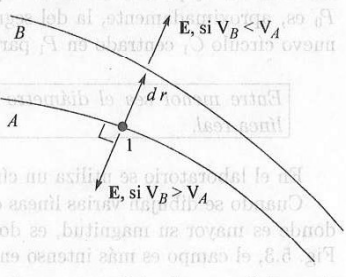
\includegraphics[width=0.4\textwidth]{practice-3/figures/campo.png}
    \caption{Relación geométrica entre equipotenciales y campo eléctrico. \\ }
    \label{fig:campo}
\end{wrapfigure} 


Sean dos superficies $A$ y $B$ a potenciales constantes $V_A$ y $V_B$ respectivamente, separadas por una distancia diferencial $dr$ (Fig. \ref{fig:campo}); las superficies se han representado con líneas; la diferencia de potencial entre estas superficies es $dV = V_B - V_A$.

La dirección del campo eléctrico $\boldsymbol{E}$ en el punto $1$ sobre $A$ es la del trayecto en el que se recorre la mínima distancia $dr$ para ir hasta $B$. Como $dV$ es positivo, entonces \begin{equation}\label{eq:gradient}
    E = -\frac{dV}{dr}\,.
\end{equation}

La dirección de $\boldsymbol{E}$ es en la dirección en que $|dV/dr|$ es máximo, o lo que lleva a que $E \perp A$. El signo $(-)$ es opuesto a la dirección en que $V$ aumenta.

Si una superficie conductora se mantiene a cierto potencial, el campo eléctrico es perpendicular a dicha superficie, precisamente por la relación de ortogonalidad entre superficies equipotenciales y líneas de $\boldsymbol{E}$.

\subsubsection{Método experimental para trazar una línea de campo}
\label{sssec:metodo}

En el laboratorio no medimos diferenciales de voltaje $dV$ ni de distancia $dr$, sino diferencias finitas $\Delta V$ y $\Delta r$.

Para trazar una línea de $\boldsymbol{E}$ nos basamos en que

\begin{center}
La máxima variación $\Delta V$, con $\Delta r$ fijo, se presenta en la dirección de $\boldsymbol{E}$.
\end{center}



Para saber la dirección de $\boldsymbol{E}$ en un punto $P_0$ (Fig. \ref{fig:proceso}), centramos una de las puntas de un multímetro en $P_0$. Después recorremos con la otra punta el perímetro de un círculo $C_0$ centrado en $P_0$ para determinar el punto $P_1$ donde $\Delta V$ es máximo. La dirección de $\boldsymbol{E}$ en $P_0$ es, aproximadamente, la del segmento $P_0P_1$. Luego repetimos el procedimiento con un nuevo círculo $C_1$ centrado en $P_1$ para hallar un punto $P_2$, y así sucesivamente.


\begin{center}
Entre menor sea el diámetro del círculo, más se aproxima la línea de $\boldsymbol{E}$ a la línea real.
\end{center}

En el laboratorio se utiliza un círculo de 2.4 cm de diámetro.

\begin{figure}[H]
    \centering

    \begin{minipage}{0.45\textwidth}
        \centering
        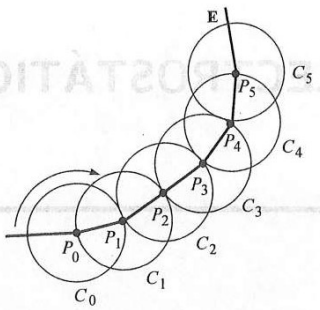
\includegraphics[width=0.6\textwidth]{practice-3/figures/proceso.png}
        \caption{Método para trazar una línea de $\boldsymbol{E}$. Se explora $\Delta V$ entre $P_i$ y el perímetro $C_i$.}
        \label{fig:proceso}
    \end{minipage}
    \hfill
    \begin{minipage}{0.45\textwidth}
        \centering
        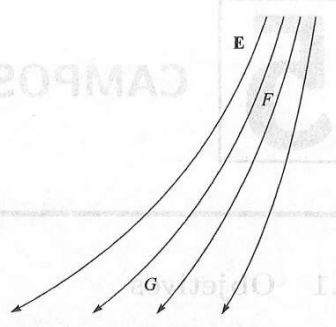
\includegraphics[width=0.6\textwidth]{practice-3/figures/campos.png}
        \caption{La magnitud de $\boldsymbol{E}$ es variable. En $F$ es mayor que en $G$.}
        \label{fig:campos}
    \end{minipage}

\end{figure}

Cuando se dibujan varias líneas de $\boldsymbol{E}$, las regiones donde el campo es más intenso, o sea donde es mayor su magnitud, es donde hay mayor densidad de líneas. Por ejemplo, en la Fig. \ref{fig:campos}, el campo es más intenso en la región $F$ que en la región $G$.

\subsubsection{Campo Eléctrico dentro de un Conductor y de un Aislante}

Si la carga de un electrón, de conducción en un metal es $-e$, y el electrón está en presencia de un $\boldsymbol{E}$, el electrón acelera pues la fuerza sobre él es $F = -eE$. O sea que donde haya electrones y campo eléctrico, necesariamente hay corriente eléctrica. Por lo tanto, dentro de un conductor, en condiciones estáticas, $E = 0$, pues si fuera diferente de cero habría movimiento de cargas y la situación no sería estática o de equilibrio: $F \ne 0$. En cambio, en un aislante, puesto que no tiene electrones de conducción, aunque $E$ sea diferente de cero no se presentan corrientes. Reemplazando en la ec. \eqref{eq:gradient} el valor de $\boldsymbol{E}$ dentro de un conductor sin corrientes eléctricas, $0 = -dV/dr$; de donde $dV = 0$. Esto quiere decir que $V$ es constante: si un conductor está a cierto potencial, todo su interior estará al mismo potencial.

% \rule{\textwidth}{1pt}

% \section*{Materiales}

% \begin{itemize}
% \item Cubeta electrostática
% \item Generador de señales (Leader)
% \item Multímetro digital (Fluke)
% \item Cables banana-caimán y caimán-caimán
% \item Cuña de aluminio
% \item Círculo transparente plástico (diámetro $\approx 2.4$ cm)
% \item Cilindro de aluminio (5 cm) y cilindro de PVC (5 cm)
% \item Regla o cinta métrica pequeña
% \end{itemize}

% \textbf{Observación importante:}
% Para evitar la electrólisis del agua que distorsionaría las mediciones con corriente continua, se utiliza una señal alterna a una frecuencia de 1000 Hz. La situación se sigue tratando como estática, y el multímetro debe configurarse para medir voltaje alterno ($V_{rms}$). Se recomienda encender el generador 8 minutos antes de iniciar para estabilizar la señal.

% \rule{\textwidth}{1pt}



% \subsection*{Procedimiento}

% \begin{itemize}
% \item Conectar la cuña exterior y el electrodo externo con un cable caimán-caimán para garantizar que sean equipotenciales.
% \item Ajustar el generador a 1000 Hz (onda senoidal) al máximo voltaje.
% \item \textbf{Trazado de equipotenciales:} Colocar una punta del multímetro (COM) en el electrodo central. Con la otra punta, buscar puntos en el agua que marquen el mismo voltaje a distintas posiciones radiales. Unir los puntos para visualizar la superficie equipotencial.
% \item \textbf{Trazado de líneas de campo:} Colocar el disco transparente en el fondo de la cubeta junto a la cuña externa. Posicionar una punta del multímetro en el centro del disco ($P_0$). Explorar el perímetro del disco con la otra punta hasta encontrar el punto de máxima diferencia de potencial ($P_1$). La línea $P_0-P_1$ marca la dirección del campo. Repetir moviendo el centro del disco a $P_1$, trazando la trayectoria hacia el electrodo central.
% \item \textbf{Análisis de materiales:} Manteniendo la referencia en el electrodo central, desplazar la punta de prueba sobre y dentro de la cuña de aluminio, el cilindro de aluminio y el cilindro de PVC (previamente depositados en el agua). Registrar las variaciones de voltaje.
% \end{itemize}

\subsection{Procedimiento}

Encienda el generador sin armar el montaje de la Fig. \ref{fig:montaje1}, y espere cerca de 8 minutos para empezar a tomar datos, mientras se estabiliza la amplitud de la señal de salida. Seleccione una frecuencia de 1000 Hz (lea el pie de página) poniendo la perilla de frecuencia en 10, y el multiplicador de rango de frecuencia en $\times 100$; ponga el máximo voltaje llevando el rango de voltaje a HIGH y rotando la perilla de FINE completamente a la derecha; seleccione una señal senoidal con el conmutador de forma de onda WAVEFORM.

Lleve el selector del multímetro a la posición para medir voltajes alternos; utilice las escalas COM y V$\Omega$.

Arme el dispositivo de la Fig. \ref{fig:montaje1}. Para asegurarse de que el electrodo externo y la cuña sean equipotenciales, conéctelos con un cable caimán-caimán. La cuña debe estar muy bien centrada entre las líneas $L_2$ y $L_6$. En la cubeta debe haber agua hasta una profundidad de 1 cm, correspondiente a la altura del primer escalón del electrodo central de aluminio.

\begin{figure}[H]
    \centering
    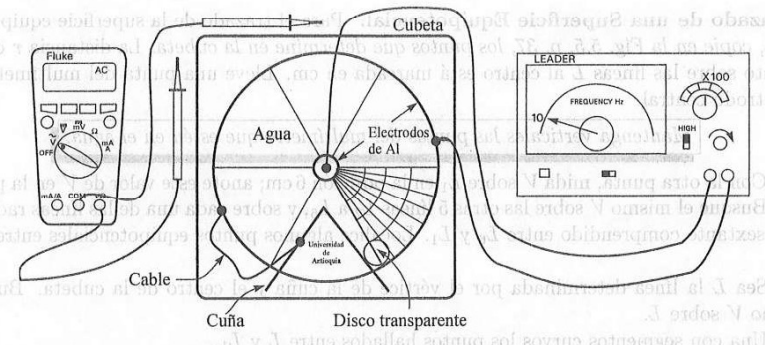
\includegraphics[width=0.5\linewidth]{practice-3/figures/montaje.png}
    \caption{Montaje experimental de la actividad I.}
    \label{fig:montaje1}
\end{figure}

\bigskip\textbf{Trazado de una Superficie Equipotencial.} Para el trazado de la superficie equipotencial, copie en la Fig. \ref{fig:diagrama1}, los puntos que determine en la cubeta. La distancia $r$ de un punto sobre las líneas $L$ al centro está marcada en cm. Lleve una punta del multímetro al electrodo central.

\begin{center}
\fbox{Mantenga verticales las puntas del multímetro que estén en el agua.}
\end{center}

Con la otra punta, mida $V$ sobre $L_1$ en la posición 6 cm; anote este valor de $V$ en la p. 37. Busque el mismo $V$ sobre las otras 5 líneas $L_2$ a $L_6$, y sobre cada una de las líneas radiales del sextante comprendido entre $L_6$ y $L_1$. Localice algunos puntos equipotenciales entre $L$ y $L_6$.

Sea $L$ la línea determinada por el vértice de la cuña y el centro de la cubeta. Busque dicho $V$ sobre $L$.

Una con segmentos curvos los puntos hallados entre $L$ y $L_1$.

Como la equipotencial debe ser simétrica respecto a $L$, copie simétricamente la curva trazada entre $L$ y $L_1$ en el sector comprendido entre $L_4$ y $L$.

Cierre o complete la equipotencial teniendo en cuenta los puntos sobre $L_1$, $L_2$ y $L_3$.

\bigskip\textbf{Trazado de una Línea de Campo Eléctrico.} Deposite en el fondo de la cubeta, sobre una de las líneas $L$, el círculo transparente. Lea su diámetro sobre la misma línea. Anote el radio en el cuadro \ref{tab:campo_electrico}.

\begin{table}[H]
\centering
\caption{Trazado de una Línea de Campo Eléctrico (Gradiente de Potencial)}
\label{tab:campo_electrico}
\begin{tabular}{|c|c|c|c|c|c|}
\hline
\textbf{Punto} & \textbf{Posición $r$} & \textbf{Potencial $V$} & \textbf{Diferencia $\Delta V$} & \textbf{Radio disco} & \textbf{Magnitud $E$} \\
$P_i$ & [cm] & [V] & [V] & $\Delta r$ [cm] & $\approx \Delta V / \Delta r$ [V/cm] \\ \hline
$P_0$ & & & --- & --- & --- \\ \hline
$P_1$ & & & & & \\ \hline
$P_2$ & & & & & \\ \hline
$P_3$ & & & & & \\ \hline
$P_4$ & & & & & \\ \hline
$P_5$ & & & & & \\ \hline
\end{tabular}
\end{table}

Aplique el método descrito en la sección \ref{sssec:metodo} para trazar líneas de campo: Coloque el círculo contra la cuña y el electrodo externo, y sobre el sextante reticulado; $P_0$ es el centro del disco. Vaya copiando en la Fig. \ref{fig:diagrama1} los puntos $P_i$ que halle en la cubeta. Una punta del multímetro manténgala vertical sobre $P_0$, y con la otra, también perpendicular al agua, explore el perímetro del círculo. Halle $P_1$ y anote el máximo $\Delta V$ entre $P_0$ y $P_1$ en el cuadro \ref{tab:campo_electrico}. Desplace el centro del círculo a $P_1$ y repita el procedimiento para hallar $P_2$, y así sucesivamente hasta llegar al electrodo central. Una los puntos hallados. Aplique el hecho de que $\mathbf{E}$ estático es perpendicular a una superficie metálica, para prolongar los extremos de la línea de $\mathbf{E}$ hasta el aluminio.

Como se está aplicando una señal de $\sim 1000$ Hz entre los electrodos, $\mathbf{E}$ va dirigido, en un segundo, 1000 veces en un sentido y 1000 veces en el sentido opuesto; por esto no se puede asignar un sentido único a la línea que acaba de trazar.

Según el cuadro del informe, ¿en qué segmento es más intenso $\mathbf{E}$ (vea la Ec. \eqref{eq:gradient})? ¿Se espera que $\mathbf{E}$ sea más intenso cerca del electrodo interno o del electrodo externo (vea la Fig. \ref{fig:campos})?

Según la Fig. \ref{fig:diagrama1}, ¿es $\mathbf{E}$ perpendicular a la superficie equipotencial? Si $\mathbf{E}$ no es perpendicular a la equipotencial, ¿cuál es la causa principal? (vea los recuadros de la Sección \ref{sssec:metodo})

\bigskip\textbf{$\mathbf{E}$ dentro de un Conductor y de un Aislante.} Lleve una punta del multímetro al electrodo central; desplace la otra punta sobre la cuña y dentro de ella; lea permanentemente la diferencia de potencial marcada por el multímetro. Según la Ec. \eqref{eq:gradient}, ¿cuánto vale $\mathbf{E}$ dentro de la cuña metálica?

Deposite en lugares arbitrarios dentro de la cubeta los cilindros de aluminio y de PVC; repita con ellos el párrafo anterior.

Retire los cilindros y el disco. Apague el generador y el multímetro.

\subsection{Análisis de datos}

\begin{itemize}
\item Graficar en papel las posiciones obtenidas para reconstruir la geometría de las superficies equipotenciales y la trayectoria de la línea de campo.
\item Verificar geométricamente si se cumple la condición de ortogonalidad $\mathbf{E} \perp V$.
\item Comparar los gradientes espaciales del voltaje ($dV/dr$) observados en el exterior versus el interior de los cilindros.
\end{itemize}

\subsection{Análisis adicional}

\begin{itemize}
\item Interpretar el significado físico del cambio (o ausencia de cambio) de voltaje al mover la punta del multímetro en el interior del cilindro de aluminio comparado con el de PVC.
\item Discutir el efecto geométrico que introduce la cuña de aluminio sobre las líneas de campo del montaje.
\item Evaluar el error introducido por el tamaño del disco transparente en la determinación de la línea de campo eléctrico.
\end{itemize}

\subsection{Resultados esperados}

\begin{itemize}
\item Mapa visual o plano esquemático de superficies equipotenciales y líneas de campo de la configuración analizada.
\item Tabla comparativa de diferencias de potencial medidas en el interior del conductor (Al) vs. el dieléctrico (PVC).
\item Verificación cualitativa de que el interior de un conductor es una región equipotencial.
\end{itemize}

\rule{\textwidth}{1pt}

% \section*{Actividad II: Verificación experimental de la Ley de Gauss}

% \textbf{Objetivo:} Determinar el campo eléctrico a distintas distancias radiales utilizando gradientes de potencial finitos y verificar la relación de conservación del flujo eléctrico en una simetría cilíndrica.

% \subsection*{Sistema experimental}

% Se utiliza la misma cubeta, pero configurada con electrodos de simetría puramente cilíndrica (un electrodo central y un aro externo concéntricos). 

% \subsection*{Procedimiento}

% \begin{itemize}
% \item Establecer 4 superficies equipotenciales concéntricas denominadas $A$, $B$, $C$ y $D$, con radios nominales $r_A = 1.5$ cm, $r_B = 2.5$ cm, $r_C = 9$ cm y $r_D = 10$ cm.
% \item Tocar el fondo de la cubeta con la punta del multímetro y medir el potencial ($V$) para cada radio a lo largo de varias líneas radiales (al menos 3 ángulos distintos).
% \item Promediar los valores de potencial y asegurar que las mediciones correspondan efectivamente a superficies equipotenciales concéntricas.
% \end{itemize}

% \subsection*{Análisis de datos}

% Para la región interna (entre $A$ y $B$):
% \begin{itemize}
% \item Calcular $\Delta r_1 = r_B - r_A$ con su respectivo error instrumental.
% \item Calcular la diferencia de potencial $\Delta V_1 = V_B - V_A$ considerando un error instrumental del 1.5\% (especificación típica del Fluke en AC).
% \item Definir el radio medio $r_1 = (r_A + r_B)/2$.
% \item Estimar la magnitud del campo en $r_1$ mediante: $E_1 \approx |\Delta V_1 / \Delta r_1|$.
% \item Calcular el producto $E_1 \cdot r_1$ y su error propagado.
% \end{itemize}

% Para la región externa (entre $C$ y $D$):
% \begin{itemize}
% \item Repetir los cálculos para hallar $\Delta r_2$, $\Delta V_2$, $r_2$, $E_2$ y el producto $E_2 \cdot r_2$.
% \end{itemize}

% \subsection*{Análisis adicional}

% \begin{itemize}
% \item Comparar los productos $(E_1 \cdot r_1)$ y $(E_2 \cdot r_2)$.
% \item Aplicar el criterio de igualdad considerando los intervalos de error calculados.
% \item Discutir el significado físico del cumplimiento o incumplimiento empírico de la ecuación \eqref{eq:Gauss_toroide} (ausencia o presencia de carga neta en la región de agua analizada).
% \item Evaluar el impacto de la polarización del agua o efectos de borde en la precisión del experimento.
% \end{itemize}

% \subsection*{Resultados esperados}

% \begin{itemize}
% \item Tablas de voltajes medidos a distintas posiciones radiales.
% \item Valores calculados del campo eléctrico para las regiones interna ($E_1$) y externa ($E_2$).
% \item Validación matemática de la relación teórica emanada de la Ley de Gauss para cilindros concéntricos ($E_1 r_1 = E_2 r_2$).
% \end{itemize}

% \rule{\textwidth}{1pt}

% \section*{Preguntas orientadoras}

% \begin{itemize}
% \item ¿Qué relación geométrica existe entre la dirección del campo eléctrico y las superficies de potencial constante?
% \item Al realizar mediciones de voltaje en el interior del cilindro de aluminio, ¿por qué el resultado se mantiene constante a pesar de la presencia del campo exterior?
% \item ¿Qué diferencia física fundamental evidencia el multímetro cuando la punta entra al cilindro de PVC en comparación con el cilindro de aluminio?
% \item ¿Por qué la magnitud del campo eléctrico decrece a medida que nos alejamos del electrodo central en esta configuración particular?
% \item ¿Cómo confirma el experimento que el flujo del campo eléctrico a través de una superficie gaussiana que no encierra carga neta es igual a cero?
% \item ¿Qué fuentes de error afectan principalmente el cálculo indirecto del campo eléctrico ($E \approx \Delta V / \Delta r$)?
% \end{itemize}

% \rule{\textwidth}{1pt}

% \section*{Conclusión esperada}

% Al finalizar la práctica, el estudiante deberá ser capaz de visualizar fenómenos electrostáticos abstractos mediante el mapeo de variables medibles macroscópicamente, como el potencial eléctrico. Deberá comprender e identificar experimentalmente el comportamiento diferenciado de los campos eléctricos en la frontera y el interior de medios conductores y dieléctricos. Asimismo, integrará el concepto de gradiente de potencial con el tratamiento del error experimental para validar de manera empírica postulados teóricos fundamentales del electromagnetismo, específicamente la Ley de Gauss y la conservación del flujo eléctrico en geometrías de alta simetría.